\documentclass[twocolumn]{article}


% Packages for TR Template
\usepackage{mathpazo}
\usepackage{microtype}


% Document packages
\usepackage[T1]{fontenc} % Use 8-bit encoding that has 256 glyphs
\usepackage{fourier} % Use the Adobe Utopia font for the document - comment this line to return to the LaTeX default
\usepackage[english]{babel} % English language/hyphenation
\usepackage{amsmath,amsfonts,amsthm} % Math packages
\usepackage{natbib} % Natural bibliography styles
%\usepackage{fullpage}
\usepackage{hyperref}
\usepackage{color}
\usepackage{booktabs}
\usepackage{listings}
\usepackage{graphicx}
\usepackage{acronym} % Used for defining acronyms


% Define acronyms
\acrodef{lda}[LDA]{Latent Dirichlet allocation}
\acrodef{csv}[CSV]{Comma Seperated Values}
\acrodef{acm}[ACM]{Association of Computing Machinery}
\acrodef{ec}[EC]{ACM Exemplar Courses}
\acrodef{ai}[AI]{Artificial Intelligence}


% Set numbering styles
\numberwithin{equation}{section} % Number equations within sections (i.e. 1.1, 1.2, 2.1, 2.2 instead of 1, 2, 3, 4)
\numberwithin{figure}{section} % Number figures within sections (i.e. 1.1, 1.2, 2.1, 2.2 instead of 1, 2, 3, 4)
\numberwithin{table}{section} % Number tables within sections (i.e. 1.1, 1.2, 2.1, 2.2 instead of 1, 2, 3, 4)


% Construct page dimensions
\setlength\textwidth{7in}
\setlength\textheight{9.5in}
\setlength\oddsidemargin{-0.25in}
\setlength\topmargin{-0.25in}
\setlength\headheight{0in}
\setlength\headsep{0in}
\setlength\columnsep{18pt}
\sloppy


% Define any custom commands
\newcommand{\eref}[1]{Equation~\ref{#1}}
\newcommand{\sref}[1]{Section~\ref{#1}}
\newcommand{\fref}[1]{Figure~\ref{#1}}
\newcommand{\tref}[1]{Table~\ref{#1}}
\newcommand{\lref}[1]{Listing~\ref{#1}}
\newcommand{\ie}{i.e.,}
\newcommand{\eg}{e.g.,}


\begin{document}

\title{
\vspace{-0.5in}\rule{\textwidth}{2pt}
\begin{tabular}{ll}\begin{minipage}{4.75in}\vspace{6px}
\noindent\LARGE Department of Computer Science\\
\vspace{-12px}\\
\noindent\large George Mason University\qquad Technical Reports
\end{minipage}&\begin{minipage}{2in}\vspace{6px}\small
4400 University Drive MS\#4A5\\
Fairfax, VA 22030-4444 USA\\
http:/$\!$/cs.gmu.edu/\quad 703-993-1530
\end{minipage}\end{tabular}
\rule{\textwidth}{2pt}\vspace{0.25in}
\LARGE \bf
Unsupervised Academic Curricula Evaluation Through Topic Modeling
}

\date{\today}

\author{
{\bf Jean Michel Rouly}\\
jrouly@gmu.edu
\and
{\bf Huzefa Rangwala}\\
rangwala@cs.gmu.edu
\and
{\bf Aditya Johri}\\
ajohri3@gmu.edu
}

\maketitle


%----------------------------------------------------------------------------
% Abstract
%----------------------------------------------------------------------------

\begin{abstract}

Identifying the concepts covered in a university course based on a high level description is a necessary step in the evaluation of a university's program of study.
To this end, data describing university courses is readily available on the Internet in vast quantities.
However, understanding natural language course descriptions requires manual inspection and, often, implicit knowledge of the subject area.
Additionally, a holistic approach to curricular evaluation involves analysis of the prerequisite structure within a department, specifically the conceptual overlap between courses in a prerequisite chain.
In this work we apply existing topic modeling techniques to sets of course descriptions extracted from publicly available university course catalogs.
%We limit the scope of this work to Computer Science departments in order to focus the number of possible topics and to allow benchmarking against third party expectations published within the field.
The inferred topic models correspond to concepts taught in the described courses.
The inference process is unsupervised and generates topics without the need for manual inspection.
We present an application framework for data ingestion and processing, along with a user-facing web-based application for inferred topic presentation.
The software provides tools to view the inferred topics for a university's courses, quickly compare departments by their topic composition, and visually analyze conceptual overlap in departmental prerequisite structures.
\end{abstract}



%----------------------------------------------------------------------------
% Introduction
%----------------------------------------------------------------------------

\section{Introduction}
\label{sec:introduction}

%------------------------------------------------

Computer Science education is an increasingly important field of growth at many universities~\cite{zweben2011,klawe2005}.
As departments grow and change, it becomes necessary to automate the comparison and evaluation processes.
However, much of the published data about departments is non-standard, natural language text that is not easy to process automatically.
There are many parties impacted by the lack of up to date, automatic, and simple to understand information about the characteristics of universities across the country.

%------------------------------------------------

Prospective college students and their parents seek out information on college courses to compare curricula in a meaningful way, based on content, in order to find their best fit.
A typical approach to this task is an information gathering and subsequent program comparison process duplicated many thousands of times across the population of rising college-going freshmen.
Hewner~\cite{hewner2014} conducted a qualitative study of CS students and found that students in CS need to make a variety of decisions about what courses they take.
Invariably, they have limited knowledge when making these decisions.
They also often make these decisions based on whether the classes will be enjoyable and assumed that since courses are required, they will have useful content.
We believe that a system such as ours can assist students with making more strategic goal-oriented decisions which many of the students want to take.
It will also allow them to better see the connection between courses and if possible make decision based on the skillset they want to develop.

%------------------------------------------------

Additionally, accrediting bodies (\eg\ ABET) typically require a department to cover a given set of standardized topics as a criterion for evaluation~\cite{ABET2015}.
The accreditation process can take up to 18 months to complete~\cite{ABET2015}; automating the departmental evaluation process would greatly reduce time spent measuring a CS department's coverage of a specific set of areas.

%------------------------------------------------

Programs of study at institutions of higher education can be represented as a chain composed of the courses required to complete a degree.
These component courses in turn are composed of the topics or concepts they are intended to cover.
Evaluation of the courses within a particular program is necessary for the evaluation of an overall academic curriculum.
Analyzing the structure of a program's prerequisite chain, for example, requires an understanding of each constituent course and any overlap of covered topics between courses and their prerequisites.
Additionally, inter-institutional curricular comparison requires an aggregate evaluation of the courses within each institution's program.
However, comparing and evaluating different courses requires expert knowledge in the relevant field.
No two courses can be measured for similarity based only on inherent, measurable properties.
A domain expert is required to inspect the description of the courses and determine their conceptual overlap.

%------------------------------------------------

Automating the information retrieval process to identify core concepts covered in any particular course removes the need for a domain expert.
By analyzing course descriptions from a corpus spanning fields and institutions, topic modeling can provide a method to generate a statistical representation of core course concepts.
Specifically, unsupervised latent variable models present a method of identifying the core concepts (\ie\ topics) covered in a course.
This introduces the possibility of applications in automated course and program evaluation methods.
The form of topic modeling employed in this work is \acf{lda}~\cite{Blei2003}.
As with any automated process of information retrieval, our proposed application of \ac{lda} comes with a certain set of limitations, discussed in \sref{sec:limitations}.

%------------------------------------------------

The overall goal of this work is the development of a system to digest large quantities of university course information, specifically academic course descriptions, and to process and ultimately generate interactive descriptions of the core concepts covered within institutional programs as illustrated by inferred topics.
Learned topics will be presented in a web-based application allowing inspection from multiple perspectives.

%------------------------------------------------




%----------------------------------------------------------------------------
% Background Information
%----------------------------------------------------------------------------

\section{Background on LDA}
\label{sec:background}

%------------------------------------------------

Topic modeling, a form of latent variable modeling, is an unsupervised machine learning method which attempts to recreate the distribution of so-called ``topics'' an author used to generate a corpus of documents.
The term topic is used to describe a frequency distribution of terms within a vocabulary.
In this use, a topic can be understood to represent an academic concept covered within the context of a course.
This is based on the assumption that the words used in a course description when introducing the course's topics are the same words used within descriptions of the topic itself.
The topics discovered in a corpus can be used to categorize documents and provide structure to an otherwise unknown dataset.

%------------------------------------------------

\acf{lda} is a specific type of topic modeling which assumes that a mixture of multiple topics exist within a single document in some proportion (\ie\ were used to generate that document)~\cite{Blei2003}.
\ac{lda} assumes a generative process where, for each word in the document, the algorithm selects a distribution over topics, selects a topic, and then selects a vocabulary term~\cite{Blei2003}.
Reversing this generative process is significantly more difficult because the topic distributions are unknown; these unknown information is what the ``hidden model'' or ``latent model'' refers to.

%------------------------------------------------

The computation \ac{lda} performs is the determination of the topic distributions over a set of documents.
Given the set of documents as input, generating the corpus topics is a probabilistic process.
Taking the variables $\theta_{d,k}$ (topic proportion for topic $k$ in document $d$), $\beta_{1:k}$ (topic $k$), $z_{d,n}$ (topic assignment for word $n$ in document $d$), and $w_{d,n}$ (the $n^{th}$ word in document $d$), \ac{lda} estimates the posterior probability in \eref{eq:posterior}~\cite{Blei2012}.

%------------------------------------------------

\begin{equation}
p(\beta_{1:K}, \theta_{1:D},z_{1:D} | w_{1:D}) = \frac{\beta_{1:K},
\theta_{1:D},z_{1:D}, w_{1:D}}{w_{1:D}}
\label{eq:posterior}
\end{equation}

%------------------------------------------------

\noindent
Gibbs Sampling is used to estimate the denominator (\ie\ the evidence)~\cite{Blei2003}.
Running \ac{lda} over a document set results in a usable set of vocabulary frequency distributions or topics for each document.

%------------------------------------------------

A graphical ``plate'' diagram of \ac{lda}'s generative process is given in \fref{fig:lda-plates}, adapted from~\cite{Blei2003}.
Circular nodes represent random variables while rectangular plates represent duplication.
The shaded node is the only observed (\ie\ evidence) variable, words from the document set.

%------------------------------------------------

\begin{figure}
  \centering
  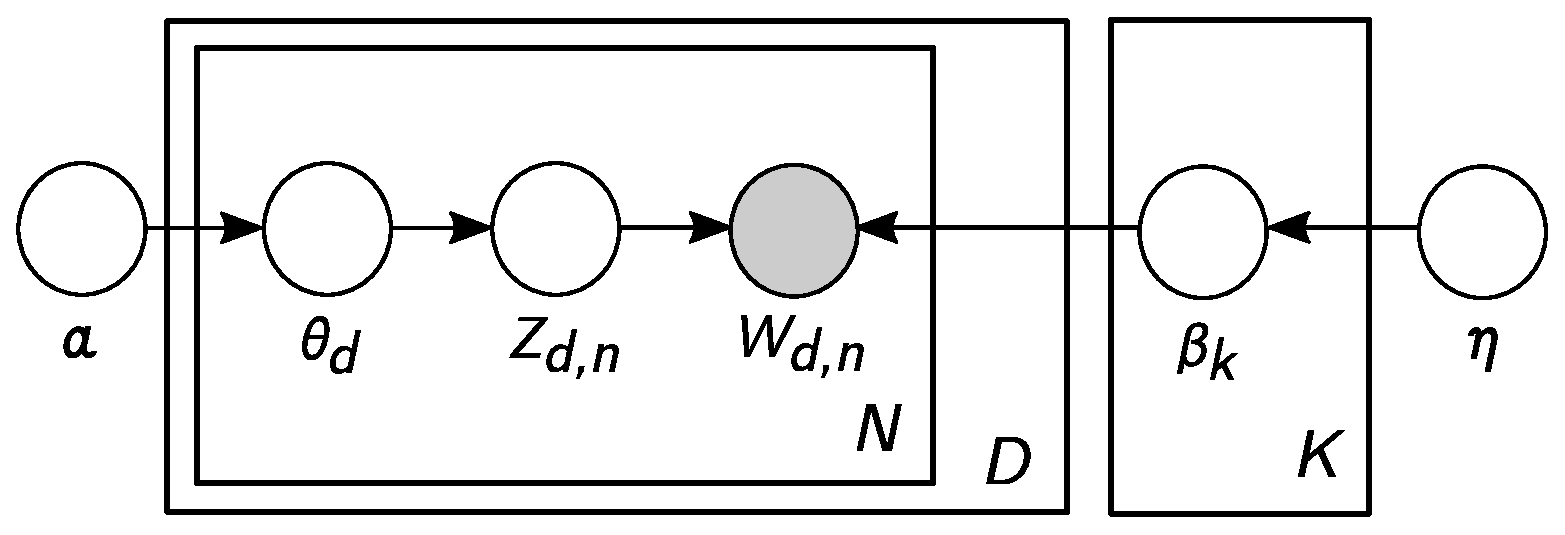
\includegraphics[width=0.45\textwidth]{figures/lda-plates}
  \caption{LDA graphical diagram adapted from~\cite{Blei2012}\label{fig:lda-plates}.}
\end{figure}

%------------------------------------------------

\subsection{Related Work}
\label{sec:related-work}

%------------------------------------------------

Our research complements other efforts within Computer Science education that are directed towards categorization of content to improve pedagogy, \eg\ Hubwieser et al.~\cite{hubwieser2013}.
We believe that our project contributes both, by identifying content (\ie\ topics) being taught across institutions and by identifying gaps and unique contributions.
This information can be compared to teacher competencies and used to design assessment and instruments to measure them.
Another area in which this work can assist is in identification of concepts and their classification, especially ``threshold concepts''~\cite{ShinnersKennedyFincher2013}.
Overall, we believe our data-driven approach complements other qualitative efforts by building on them and by automating some aspects of the research.
The work of~\cite{airasian2001taxonomy} discusses a taxonomy related to learning breaking the process down along the cognitive process and knowledge dimensions.
Using a richer source of course information that course descriptions our proposed method could be adopted to learn concepts along these dimensions.

%------------------------------------------------

Other work has also attempted to extract concept information from course data.
Yang et al.\ employ four distinct techniques to map courses into a conceptual space and then learn prerequisite relationships between similar courses~\cite{Yang2015}.
Two of their conceptual mapping techniques generate latent features, which have the downside of not being human-readable as in \ac{lda}.
The remaining two techniques generate human-readable topics, but rely either on an outside source (Wikipedia) or simply represent concepts as the vocabulary of the document.
The benefit of \ac{lda} as an information retrieval tool is its ability to generate pseudo human-readable topics while acting in a fully unsupervised manner on a single, large data set.
Our approach naively targets a dataset of fixed universities and customizes web scrapers specifically for their computer science departments.
Effland et al.\ introduces a robust web crawler system to automatically search for, identify, and extract course descriptions from disparate locations on the Internet~\cite{Effland2015}.
Application of similar technology in this work was considered, and would greatly improve the scale of the analyzed data.

%------------------------------------------------




%----------------------------------------------------------------------------
% Methods
%----------------------------------------------------------------------------

\section{Methods}
\label{sec:methods}

%------------------------------------------------

The structure of this work is threefold.
First, a dataset of university course descriptions is generated using publicly available data from a number of North American universities.
This process is discussed in \sref{sec:data-acquisition}.
Second, \ac{lda} is applied to the collected data and topics are inferred.
This step is discussed in \sref{sec:topic-modeling}.
Finally, the collected data and inferred topics are presented in a user-facing web application, described in \sref{sec:visualization}.

%------------------------------------------------

\subsection{Data Acquisition}
\label{sec:data-acquisition}

%------------------------------------------------

The primary data manipulated in this study are university catalog course descriptions.
The current experimental data sources are described in \tref{tbl:dataset}.
Note that only Computer Science departments are included in this dataset, in order to simplify the evaluation process and the required number of inferred topics.
Simple web scrapers were written using Python and BeautifulSoup to download publicly available descriptions from university catalogs.
These will be made publicly available at
%%%%%%%%%%%%%%%%%%%%%%%%%%%%%%%%%%%%%%%%%%%%%%%%%%%%%%%%%%%%%%%%%%%%%%%%%%%%%%
% TODO: Blind replace.
\url{http://redacted} (This will be available upon publication and is not available for blind submission).
% \url{http://github.com/jrouly/trajectory}.
%%%%%%%%%%%%%%%%%%%%%%%%%%%%%%%%%%%%%%%%%%%%%%%%%%%%%%%%%%%%%%%%%%%%%%%%%%%%%%
Descriptions and catalog webpages appear in a vast variety of different formats, structures, and HTML correctness, so a parser was written for each university to acquire the unstructured text.
This text was then passed through a cleaning procedure to remove abbreviations and non-English characters, as well as common English stop words.
Finally the text was passed through a stemmer to strip morphology from the words and eliminate duplicate terms.
At the same time, departmental course prerequisite data is collected from the catalog as well.
Prerequisites are limited to courses in the database, meaning that references older courses that are no longer present in the catalog are ignored.
Non-specific prerequisite references (\eg\ \texttt{400-level}) are ignored as well.

%------------------------------------------------

\begin{table}
  \centering
  \begin{tabular}{lcl}
    \toprule
    University & Course Count \\
    \midrule
    American University (AU) & 32 \\
    George Mason University (GMU) & 145 \\
    Kansas State University (KSU) & 83 \\
    Louisiana State University (LSU) & 59 \\
    Portland State University (PDX) & 190 \\
    Rensselaer Polytechnic Institute (RPI) & 61 \\
    University of South Carolina (SC) & 64 \\
    Stanford University (Stanford) & 69 \\
    University of Utah (Utah) & 142 \\
    University of Tennessee, Knoxville (UTK) & 29 \\
    \midrule
    \ac{ec} & 68 \\
    \bottomrule
  \end{tabular}
  \caption{CS program statistics\label{tbl:dataset}}
\end{table}

%------------------------------------------------

The Python scraping framework developed is structured to allow pluggable web scrapers tooled to specific syllabus repositories.
There are a number of existing web scrapers in place pointing to different university course catalogs, but the code can be easily extended in the future to grow the data set.
Integrated in the scraping framework is a lightweight relational database layer to store both course description data and university metadata, including names, URLs, and prerequisite information.
The database layer also stores inferred topics.

%------------------------------------------------

\subsection{Preliminary Data Exploration}
\label{sec:data-exploration}

%------------------------------------------------

In addition to \ac{lda}, other unsupervised machine learning tools can be applied to the same data set.
Simple clustering algorithms (\eg\ K-Means) when given the same bag of words corpus as input act to identify groupings of similar documents according to their term frequency vector Euclidean distance~\cite{lloyd1982}.
Additional, similar clustering algorithms can be applied in a similar manner.

%------------------------------------------------

Preliminary exploratory results are promising.
We applied K-Means clustering to a sample dataset of course descriptions selected from the George Mason University Computer Science online catalog across multiple semesters.
Using course section IDs as ground-truth labels, we clustered the course descriptions.
\tref{table:cluster-metrics} summarizes the metrics computed on the resulting clustering.
Homogeneity represents the ``same-ness'' of a cluster, or the degree to which each cluster contains only members of a single type.
Completeness represents the ``spread'' of courses across clusters, or the degree to which every member of the same type is assigned to the same cluster.
V-Measure is simply the harmonic mean of the prior two metrics.
For each metric, higher is better, and they are bounded from 0 to 1.
A distributed implementation of K-Means available in the Python toolkit \texttt{scikit-learn} was used to perform the clustering.

%------------------------------------------------

The high completeness values are promising: this indicates that many of the same course are assigned under the same cluster prototype.
The low value of homogeneity is unsurprising given the initialization parameters used: K-Means was initialized to detect only 20 clusters, a far smaller number than the magnitude of distinct course sections available.
The number 20 was chosen arbitrarily as a smaller count than the true number of distinct course sections in order to increase cluster size.

%------------------------------------------------

\begin{table}[ht]
\centering
\begin{tabular}{ll}
\toprule
Execution time & 0.144s \\
Homogeneity & 0.415 \\
Completeness & 0.877 \\
V-measure & 0.563 \\
\bottomrule
\end{tabular}
\caption{Preliminary clustering metrics\label{table:cluster-metrics}}
\end{table}

%------------------------------------------------

\subsection{Topic Modeling}
\label{sec:topic-modeling}

After the exploratory clustering process, we pass\-ed clean\-ed data into a topic modeling framework by exporting from the database layer to the filesystem in a structured ``bucket of files'' format.
The Java MALLET library is used to perform \ac{lda} on the course description data.
A data pipeline is constructed using the MALLET API that reads input data, tokenizes it, and trains an \ac{lda} topic model.
The inferred topics are then exported to a common \ac{csv} format and read back into the database layer and applied to existing courses.
Independent runs of \ac{lda} with distinct parameterization are segregated in the database into ``Result Sets'', allowing sets of inferred topics to sit side by side without interfering.
This also allows the presentation of different sets of inferred topics to the end user.

%------------------------------------------------

The initialization parameters of MALLET's \ac{lda} implementation are summarized in \tref{table:lda-parameters}.
Experiments were run varying parameters throughout the experimental range, including the MALLET default values.
However, as the number of topics increased greatly beyond 750, and as $\beta$ decreased greatly below 0.0001, the MALLET framework began to encounter instability and errors.
Any runs which encountered infinite or ``not-a-number'' values were immediately discarded.
Ultimately 77 result sets were retained for analysis.

%------------------------------------------------

\begin{table*}[ht]
\centering
\begin{tabular}{llll}
\toprule
Parameter  & Description & Experimental Range & Default \\
\midrule
$\alpha$   & Dirichlet concentration parameter. & [1, Iterations] & Iterations \\
$\beta$    & Dirichlet concentration parameter. & [0.0001, 0.5] & 0.01 \\
Iterations & The number of \ac{lda} iterations. & --- & 3000 \\
Topics     & The number of topics to infer. & [100, 1000] & --- \\
\bottomrule
\end{tabular}
\caption{LDA Initialization Parameters\label{table:lda-parameters}}
\end{table*}

%------------------------------------------------

\subsection{Visualization}
\label{sec:visualization}

%------------------------------------------------

An interactive, dynamic user visualization of course descriptions and topics has been prototyped.
The visualization is a web-based application built upon the Python Flask library.
The tool interfaces with the same database layer used by the rest of the application framework to provide an aesthetically pleasing user-facing interface with several primary modules.
By default, the web application presents the user with a high level ``dashboard'' overview of the dataset and available result sets, where a result set is the set of topics inferred after a single run of the \ac{lda} module with a distinct initialization set.
After selecting a result set, the user can browse the data by course, department, university, or inferred topics.
The remainder of this section describes implementation details of the tool's primary features.

%------------------------------------------------

\subsubsection{Explore Courses}
\label{sec:vis-course}

%------------------------------------------------

When presented with the complete university dataset, the user may interactively search for a university.
Once a university is selected, the user may search through its registered departments and select a course of interest.
On selecting a course, the text of its description is displayed in both its original format and its cleaned, stemmed format.
Additionally, the course's inferred topics are listed in order of their proportion within the course description.
These topics are expandable, and upon interaction present the user with the list of other known courses with that inferred topic.
Any topics appearing in a document with proportion under 15\% are automatically hidden from the user.
This design choice was implemented to reduce visual clutter from inferred topics with low relevance to the class.

%------------------------------------------------

\subsubsection{Prerequisite Chain Analysis}
\label{sec:vis-prerequisites}

%------------------------------------------------

In addition to the course-specific data, an interactive, collapsible tree visualization of the course' prerequisite chain is displayed.
The recursively generated tree visualization provides a high level view of the course's position within a department.
\fref{fig:prerequisite-detail} details the prerequisite tree visualization.
Above this visualization is the prerequisite chain conceptual analysis tool.
This tool automatically provides a view of any registered prerequisite courses along with their inferred topics.
Any shared topics between the prerequisites and the selected course are highlighted to indicate conceptual overlap.

%------------------------------------------------

Observe the course CS 310 ``Data Structures'' in the upper middle of the prerequisite tree.
\tref{tbl:310-topics} details its topics, along with the topics of its prerequisite courses CS 105 ``Computer Ethics and Society'' and CS 211 ``Object-Oriented Programming''.
Clearly there is a significant area of overlap between a data structures course and an introductory course in object oriented programming, as illustrated by the two italicized overlapping topics.
Specifically, the overlap is in the areas of algorithms and data structures as well as object oriented programming.
The ethics course, however, does not share any conceptual overlap with CS 310.
Inspecting the context of these courses, however, reveals that CS 105 is a common freshman requirement at George Mason, and many upper level classes depend on its completion.
It is intended as a baseline of student maturity rather than a prerequisite because of the concepts it introduces.

%------------------------------------------------

\begin{figure*}
  \centering
  \includegraphics[width=\textwidth]{figures/screenshots/course/prerequisite_detail_cropped.png}
  \caption{Interactive prerequisite tree visualization tool\label{fig:prerequisite-detail}}
\end{figure*}

%------------------------------------------------

\begin{table*}[ht!]
  \centering
  \begin{tabular}{ll}
    \toprule
    GMU CS 310 Topics & Proportion \\
    \midrule
    \emph{languag, object, program, orient, includ, type, abstract, design, implement, concept} & 29.946\% \\
    \emph{program, problem, solv, algorithm, data, structur, comput, introduct, languag, techniqu} & 21.461\% \\
    includ, design, system, topic, comput, introduct, cover, applic, algorithm, techniqu & 26.117\% \\
    \midrule
    GMU CS 211 Topics [Prerequisite] & Proportion \\
    \midrule
    \emph{languag, object, program, orient, includ, type, abstract, design, implement, concept} & 29.433\% \\
    \emph{program, problem, solv, algorithm, data, structur, comput, introduct, languag, techniqu} & 26.772\% \\
    code, compil, pars, analysi, optim, gener, languag, lexic, techniqu, construct & 18.685\% \\
    comput, method, theori, basic, principl, includ, topic, model, cover, scientif & 16.076\% \\
    \midrule
    GMU CS 105 Topics [Prerequisite] & Proportion \\
    \midrule
    ethic, comput, issu, profession, social, technolog, privaci, legal, relat, digit & 75.964\% \\
    \bottomrule
  \end{tabular}
  \caption{Topics of GMU CS 310 and its prerequisite courses, CS 105 and CS 211. Overlapping topics are italicized.\label{tbl:310-topics}}
\end{table*}

%------------------------------------------------

\subsubsection{Compare Departments}
\label{sec:vis-compare}

%------------------------------------------------

The user may also compare two university departments.
Topics inferred from every course in the department are collected and displayed side by side.
Topics unique to each department are displayed separately from the intersection set of common topics.
Similarity metrics describing the relationship between the two departments are defined as well --- Jaccard index, cosine similarity, and Euclidean distance.
Defined as $\frac{\left| A \cap B\right|}{\left| A \cup B\right|}$, the Jaccard index is based on the number of items unique to and shared between each set~\cite{jaccard1912}.
The remaining metrics are based on a ``topic-vector'' representation of each department.
The topic-vector is a binary vector where each bit indicates whether a particular topic was inferred for the given department.
Features are unweighted and the topic-vector indicates only whether a topic is present in a department's topic set, and not its frequency of occurrence.
Interpreting this vector representation geometrically, the Euclidean and cosine distances are calculated.

%------------------------------------------------

\subsubsection{Evaluate Department}
\label{sec:vis-evaluate}

%------------------------------------------------

The tool also allows users to easily evaluate university departments against third party benchmarks.
The benchmarks used in this study are the \ac{acm} Knowledge Areas.
\sref{sec:evaluation} discusses the departmental evaluation process more in depth, but the web tool automatically evaluates the performance of a university department.
The tool checks for conceptual overlap between courses and \ac{acm} Knowledge Areas and predicts Knowledge Area labels where overlap exists.
Additionally, if the department has been manually annotated with Knowledge Areas, these ``ground truth'' labels are compared against the predicted labels, and the Jaccard coefficient between the two sets is computed.

%------------------------------------------------



%----------------------------------------------------------------------------
% Evaluation
%----------------------------------------------------------------------------

\section{Evaluation}
\label{sec:evaluation}

%------------------------------------------------

The \ac{acm} maintains an annual writeup of guidelines for undergraduate computer science education.~\cite{CS2013}
These guidelines include two important sections, the \acf{ec} and Knowledge Areas.
The Knowledge Areas are 18 broad topics within Computer Science as put forth by the \ac{acm}.
\ac{ec} include real course descriptions from disparate sources compiled by the \ac{acm} and manually annotated with the Knowledge Areas they cover.
These data sets are used to perform primary evaluation.

%------------------------------------------------

Using manually annotated course descriptions (eg.\ the \ac{ec} or the George Mason University Computer Science department courses\footnote{\url{http://cs.gmu.edu/~white/Curriculum2013}}) as a ground truth label set, Knowledge Area predictions are compared against known Knowledge Areas.
Knowledge Areas prediction are made by determining which Knowledge Areas share inferred topics with each course in a department.
Evaluation is performed by computing the similarity between the predicted and ground truth Knowledge Area labels.
The label set similarity is computed in two ways.
First, the Jaccard index of the predicted and ground truth labels is calculated.
Then, the percent of the ground truth labels included in the prediction set is calculated.
The web visualization provides an automatic interface for performing this evaluation process, discussed in \sref{sec:vis-evaluate}.

%------------------------------------------------

In the sequel, three case studies are described in depth to exemplify the main features of the tool.
First, \sref{sec:eval-prerequisites} discusses the prerequisite analysis features of the tool, and presents a summary of statistics about the universities included in this study.
Second, \sref{sec:eval-topics} considers a single area within Computer Science and discusses the inferred topics for courses within that area.
Finally, \sref{sec:eval-comparison} details the similarities and differences between two university departments and also presents a summary of comparisons between all the universities in this study.

%------------------------------------------------

%\begin{table}[ht]
%\centering
%\begin{tabular}{lll}
%\toprule
%& Jaccard & Percent \\
%\midrule
%mean   & 0.145 & 0.229 \\
%median & 0.156 & 0.217 \\
%\midrule
%max    & 0.007 & 0.007 \\
%min    & 0.311 & 0.709 \\
%\bottomrule
%\end{tabular}
%\caption{Evaluation of all result sets\label{tbl:evaluation-before}}
%\end{table}

%------------------------------------------------

%\begin{table}[ht]
%\centering
%\begin{tabular}{lll}
%\toprule
%& Jaccard & Percent \\
%\midrule
%mean   & 0.203 & 0.377\\
%median & 0.206 & 0.351\\
%\midrule
%max    & 0.058 & 0.082\\
%min    & 0.311 & 0.709\\
%\bottomrule
%\end{tabular}
%\caption{Evaluation of result sets with more than one predicted knowledge area on average per course\label{tbl:evaluation-after}}
%\end{table}

%------------------------------------------------

\subsection{Case Study: Prerequisite Analysis}
\label{sec:eval-prerequisites}

%------------------------------------------------

To understand how a course fits into a department, its position in the prerequisite chain must be analyzed.
Take, for example, a course in mobile application development.
We predict that any course of this nature will most likely be an upper level elective with a moderate number of prerequisite courses.
Indeed, we see this is the case with George Mason's CS 477, Portland State's CS 410, and Stanford's 231M.
However, many of the topics covered in a mobile development course are niche topics, and specific to that field.
Therefore, it might not be the case that any particular lower level courses will cover specific, overlapping topics.

%------------------------------------------------

Let us consider George Mason University's CS 477 ``Mobile Application Development''.
The course description discusses mobile platforms and the various software design issues specific to mobile platforms.
There are two inferred topics for this course.
The first topic, with 32\% proportion, includes the terms ``develop'', ``platform'', and ``mobile'' at high frequency.
The second topic, with only 15\% proportion, is more generic and includes terms like ``system'', ``computer'', and ``topic''.
The course also has two registered prerequisites: CS 310 ``Data Structures'' and CS 367 ``Computer Systems and Programming''.
Within the context of the department, these two courses are major prerequisites for any upper level course.
As expected, neither of the two prerequisite courses share the mobile-specific topic inferred for CS 477.
CS 310, however, does overlap with the generic computer systems topic.
We therefore conclude that the CS 477 course registers its prerequisites primarily to ensure a baseline level of maturity and skill among its students, rather than because some necessary concepts are introduced at a lower level and expanded upon at the higher level.

%------------------------------------------------

To quantify the typical level of conceptual overlap between prerequisites within a department, we introduce a novel vector representation of a course, the ``weighted topic-vector''.
Like the unweighted topic-vector representation of a department, the weighted topic-vector is a vector of uniform length corresponding to the total number of inferred topics among all known courses.
However, the features of a weighted topic-vector represent the proportion with which the particular topic is represented in the course's description.
In this way, the weighted topic-vector takes into account the importance of a topic to a course, rather than simply binary topic membership as in the unweighted topic-vector.
By computing the average distance between the weighted topic-vectors of a course and its prerequisites, the level of conceptual overlap for that course can be quantified.
Averaging these distance measures over every course in the department that has registered prerequisites results in a measure of average prerequisite conceptual overlap within the department.
\tref{tbl:prereq-topic-overlap} summarizes the levels of conceptual overlap for the five universities in the dataset with registered prerequisite trees, where a higher average value of conceptual overlap indicates a closer relationship between courses and their prerequisites.
The five universities not included did not have prerequisite relationships in their collected data, and thus this analysis could not be performed.

%------------------------------------------------

\begin{table}
  \centering
  \begin{tabular}{rcc}
    \toprule
     & Prereq$_\mu$ & Prereq$_\sigma$ \\
    \midrule
    GMU  & 0.324 & 0.211 \\
    AU   & 0.278 & 0.134 \\
    KSU  & 0.273 & 0.213 \\
    Utah & 0.257 & 0.249 \\
    UTK  & 0.201 & 0.256 \\
    \bottomrule
  \end{tabular}
  \caption{Level of conceptual overlap between courses and their prerequisites in five universities. Prereq$_\mu$ is the average level of conceptual overlap between prerequisites, Prereq$_\sigma$ is the standard deviation.\label{tbl:prereq-topic-overlap}}
\end{table}

%------------------------------------------------

\subsection{Case Study: Ethics In Computer Science}
\label{sec:eval-topics}

%------------------------------------------------

Computer Science is a wide ranging field, with a number of disparate subfields --- according to the \ac{acm}, there are 18 distinct Knowledge Areas.~\cite{CS2013}
At any given university, the Computer Science department will, ideally, cover all or most of these areas.
One particular area covered by most universities in this study is ``Social Issues and Professional Practice''.
A clear example of a course within this Knowledge Area is any course in computing and ethics.
Take, for example, Kansas State's CIS 415 ``Ethics and Computing Technology.''
The description is brief and to the point, focusing on computing ethics within a professional context.
The only topic inferred for this course, at 64\% proportion, includes the terms ``ethics'', ``computer'', ``profession'', ``issue'', and ``social'' at high frequency.
Searching for other courses that teach to the same topic yields 30 courses across nine universities (every university in the study except for Rensselaer Polytechnic).
These courses have titles like ``Computer Ethics and Society'' (GMU CS 105) and ``Ethics in Computing'' (LSU CSC 1200).
This demonstrates the ability of our tool to not only automatically infer relevant concepts from a course description, but to match related courses across universities.

%------------------------------------------------

\subsection{Case Study: George Mason vs Stanford}
\label{sec:eval-comparison}

%------------------------------------------------

While institutions generally cover a wide range of topics, there are always certain topics that cannot be or are not taught.
Take for example George Mason University and Stanford University.
The two computer science departments share a lot in common.
Of 68 total topics covered between the two, 41 are common to both while only 14 are unique to Stanford and 13 unique to George Mason.
The shared topics contain terms that directly relate to similar courses at each school.
For example ``secure'' and ``network'' are terms in a topic taught in network security classes at both schools.
However, a topic containing ``linux'', ``unix'', ``lab'' appears unique to Stanford, covered by CS 1U ``Practical Unix'', a course that does not exist at George Mason.
Similarly, a topic containing ``parallel'' and ``algorithm'' appears unique to George Mason.
The course GMU CS 683 ``Parallel Algorithms'' teaches to this topic, with no analogous course at Stanford.

%------------------------------------------------

By analyzing the set of unique and shared topics within two departments, simple coefficients can be computed to quantify the degree of similarity.
The Jaccard coefficient is computed as the most basic representation of departmental similarity, along with Euclidean and cosine similarity metrics discussed in \sref{sec:vis-compare}.
A pairwise comparison of the universities in this study is presented in \fref{fig:heatmap}.
In this figure, darker shades of blue represent a higher degree of similarity.
Also note that the \ac{ec} are included in this diagram as a benchmark set of courses.

%------------------------------------------------

\begin{figure}
  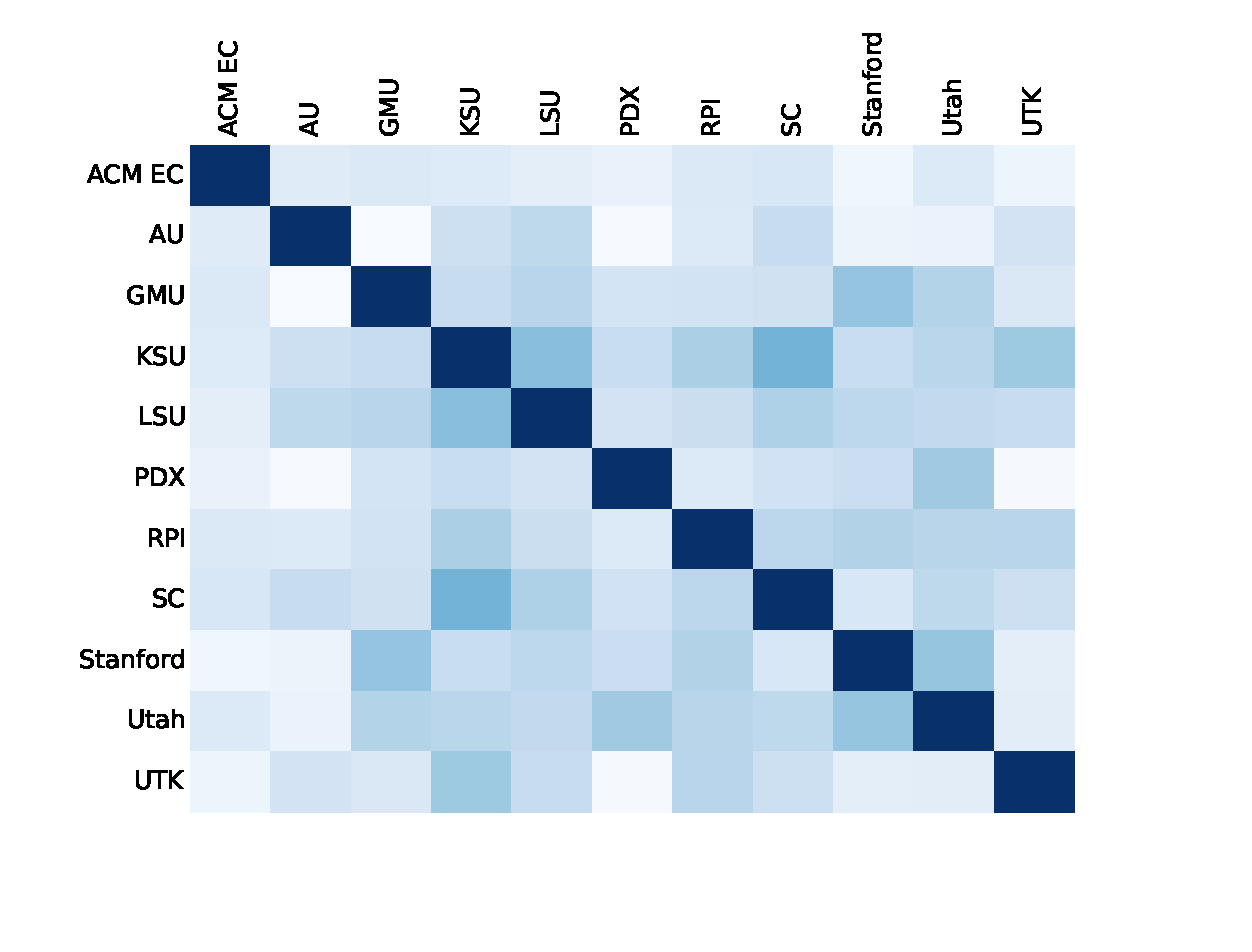
\includegraphics[width=0.5\textwidth]{figures/10by10heatmap}
  \caption{Pairwise similarity of CS departments using the Jaccard index. Darker shades indicate higher similarity. ACM EC refers to the \acf{ec}. (\sref{sec:evaluation})\label{fig:heatmap}}
\end{figure}

%------------------------------------------------



%----------------------------------------------------------------------------
% Discussion
%----------------------------------------------------------------------------

\section{Discussion}
\label{sec:discussion}

%------------------------------------------------

The preliminary results of this study have been positive.
Exploratory K-Means clustering resulted in clusters with a high level of completeness.
Even superficial manual analysis of clusters indicated that the collected data were being appropriately grouped.
Similar findings were encountered after the application of \ac{lda} topic modeling.

%------------------------------------------------

Inferred topics generally fall into one of two categories for each course.
The first category of topic includes relevant terms and keywords found in the course description.
A highly specialized course in a particular subfield might contain a set of these topics that relate to keywords from within the specific domain of the course.
The second category of topic includes more generic words common to a large number of courses.
Topics in this category often relate to concepts common across courses, eg.\ student research or exam and project information.

%------------------------------------------------

Take, for example, a computer science course in ethics.
At George Mason University the seminal IT ethics course is CS 306.
The primary topic inferred for this course in a given Result Set might look like ``ethic, comput, issu, profession, social, impact, privaci, digit, context, technolog.''
Additionally, the prerequisite course to 306, CS 105, shares this same topic.
While the topic itself is a frequency distribution over vocabulary, and does not quantifiably evaluate to an ``ethics'' topic, manual inspection clearly shows that this topic involves ethocs and social issues as they relate to technology professionals.

%------------------------------------------------

Our confidence in the applicability of \ac{lda} as a course content inference system stems from the appearance of the same or related topics within the same or related courses.
Inspecting the same course at different institutions results in the same topics being inferred at each institution.
Inspecting prerequisite courses within the same institution illustrates the relationship between the courses by highlighting conceptual overlap, ie.\ the appearance of the same topic in both course and prerequisite.
As mentioned in \sref{sec:evaluation}, third party course descriptions act as an additional evaluative metric for this approach.
A high level of consistency is indicated by the same topics being inferred for the same course at multiple institutions, related courses within the same institution, and the third party benchmark course.

%------------------------------------------------




%----------------------------------------------------------------------------
% Future Work
%----------------------------------------------------------------------------

\section{Future Work}
\label{sec:future-work}

%------------------------------------------------

One of the major benefits and weaknesses of \ac{lda} is its unsupervised nature.
Beneficially, it allows for the extraction of information from an entirely unknown dataset.
In this context, this flexibility allows its application to any number of diverse academic departments.
However, the main drawback of this characteristic is the lack of categorical information for the inferred topics.
While a topic can be understood via manual inspection of its terms, \ac{lda} offers no single comprehensive label to summarize it.
A possible solution to this problem might involve a meta-analysis of inferred topics.
Each topic could be classified as one of a number of learning outcomes based on its composition and weighting in a description.
Mapping the learned topics onto a standardized framework of learning outcomes~\cite{krathwohl2002} would allow for immediate integration of the extracted course concepts into existing academic evaluative frameworks based on learning outcome literature.

%------------------------------------------------




%----------------------------------------------------------------------------
% Conclusion
%----------------------------------------------------------------------------

\section{Conclusion}
\label{sec:conclusion}

%------------------------------------------------

Programs of study in higher education differ widely between departments and universities.
Because of these discrepancies, program evaluation methodologies are employed with the goal of standardizing the contents of a program of study.
However, this process generally requires manual inspection by a domain expert to extract information from large quantities of course descriptions.
Automating the digestion and processing of these descriptions will greatly reduce the time and effort required.
Topic Modeling presents a statistical machine learning method to extract the hidden topics behind a document set, in this case the core concepts covered by a course description.
\acf{lda} results in a feasible breakdown of textual descriptions into component concepts.

%------------------------------------------------

% TODO: More content.

%------------------------------------------------




%----------------------------------------------------------------------------
% References
%----------------------------------------------------------------------------

\bibliographystyle{plain}
\bibliography{../bibliography/bibliography}


%----------------------------------------------------------------------------
% Appendices
%----------------------------------------------------------------------------

\appendix

%------------------------------------------------

\section{Code}
\label{app:code}

Source code of current archive is available online at \href{https://github.com/jrouly/trajectory.git}{https://github.com/jrouly/trajectory}.

%------------------------------------------------

\section{Datasets}
\label{app:datasets}

See \tref{table:data-sources} for the list of universities analyzed and the number of courses scraped from their catalogs.
Note that some universities had their entire catalog scraped (resulting in several thousand courses) while others only had the Computer Science (or comparable) department scraped.
The additional departments are only used for visualization purposes --- \ac{lda} is restricted to the Computer Science courses at each university.

\begin{table*}[ht]
\centering
\begin{tabular}{lll}
\toprule
University & Course Count & URL \\
\midrule
George Mason University & 6840 & \url{catalog.gmu.edu} \\
Portland State University & 193 & \url{pdx.edu/computer-science} \\
Kansas State University & 4045 & \url{catalog.k-state.edu} \\
Louisiana State University & 59 & \url{catalog.lsu.edu} \\
Rensselaer Polytechnic Institute & 61 & \url{catalog.rpi.edu} \\
Stanford University & 69 & \url{explorecourses.stanford.edu} \\
\bottomrule
\end{tabular}
\caption{Current data input sources\label{table:data-sources}}
\end{table*}

%------------------------------------------------




\end{document}
